\documentclass{article}


\usepackage{arxiv}

\usepackage[utf8]{inputenc} % allow utf-8 input
\usepackage[T1]{fontenc}    % use 8-bit T1 fonts
\usepackage{hyperref}       % hyperlinks
\usepackage[dvipsnames]{xcolor}
\usepackage{url}            % simple URL typesetting
\usepackage{booktabs}       % professional-quality tables
\usepackage{amsfonts}       % blackboard math symbols
\usepackage{nicefrac}       % compact symbols for 1/2, etc.
\usepackage{microtype}      % microtypography
\usepackage{lipsum}
\usepackage{fancyhdr}       % header
\usepackage{graphicx}       % graphics
\graphicspath{{figures/}}     % organize your images and other figures under figures/ folder

\hypersetup{
    colorlinks=true,
    linkcolor=teal,
    % filecolor=magenta, 
    urlcolor=magenta,
    citecolor=teal,
    % pdftitle={GD},
    % pdfpagemode=FullScreen,
    % linktoc=all
    }

\usepackage{amsmath,amsfonts,amssymb,amsthm,mathtools,esint,eucal}  %math
\usepackage{subcaption}
%Header
\pagestyle{fancy}
\thispagestyle{empty}
\rhead{ \textit{ }} 

% Update your Headers here
% \fancyhead[LO]{Running Title for Header}
% \fancyhead[RE]{Firstauthor and Secondauthor} % Firstauthor et al. if more than 2 - must use \documentclass[twoside]{article}
  
%% Title
\title{Contrastive Learning with Augmentations for Training Dialogue Embeddings.
%%%% Cite as
%%%% Update your official citation here when published 
\thanks{\textit{\underline{Citation}}: 
\textbf{Authors. Title. Pages.... DOI:000000/11111.}} 
}

\author{
  Ilya Alekseev \\
  Lomonosov Moscow State University \\
  \texttt{ilya\_alekseev\_2016@list.ru} \\
  %% examples of more authors
   \And
  Denis Kuznetsov \\
  Moscow Institute of Physics and Technology \\
  \texttt{kuznetsov.dp@phystech.edu} \\
  %% \AND
  %% Coauthor \\
  %% Affiliation \\
  %% Address \\
  %% \texttt{email} \\
  %% \And
  %% Coauthor \\
  %% Affiliation \\
  %% Address \\
  %% \texttt{email} \\
  %% \And
  %% Coauthor \\
  %% Affiliation \\
  %% Address \\
  %% \texttt{email} \\
}


\begin{document}
\maketitle


\begin{abstract}
Text embeddings from pre-trained language models have been proven to be extraordinarily useful for various sentence-level tasks, such as pair classification, similarity estimation, and retrieval. Corresponding models are usually trained on large amounts of clean and diverse data using contrastive loss. Unfortunately, there are no such datasets for the domain of dialogue data. In this work, we describe the process of mining a synthetic dataset of dialogues for contrastive learning with hard negative samples. We apply various augmentation strategies for constructing dialogues with preserved or corrupted sets of intents. We train dialogue embeddings and report its performance on transfer learning tasks: domain classification, intent similarity, dialogue retrieval.
\end{abstract}


% keywords can be removed
\keywords{text embedding \and dialogue \and augmentation \and natural language processing \and contrastive learning}


\section{Introduction}
Obtaining embeddings is one of the key tasks in machine learning and popular one in recent years, because vector representation of an object is a convenient mathematical object. If an embedding accurately and comprehensively encodes the semantics of the original data, it opens up the possibility of using it in a wide range of downstream tasks.

In the field of natural language processing, classical methods for text vectorization such as bag of words \cite{bow} and tf-idf \cite{SprckJones2021ASI} have long been discovered. Thanks to deep learning, we have witnessed remarkable word vectorization techniques such as word2vec \cite{mikolov2013efficient} and GloVe \cite{pennington-etal-2014-glove}, which convey the semantic similarity between words; CoVe \cite{mccann2018learned} and ELMo \cite{peters-etal-2018-deep}, which encode information about the surrounding context. Recently, powerful encoder models have emerged that produce general-purpose text embeddings \cite{xiao2023cpack, wang2022text, li2023general}. They incorporate so much semantic information about texts that it can be applied to tasks such as classification, clustering, ranking, semantic textual similarity, and more \cite{muennighoff2023mteb}. The success of these models is largely attributed to the use of contrastive learning on massive datasets. 

However, the more specific the data structure, the more challenging it is to mine a large dataset. Language models, such as those presented in \cite{zhang-etal-2023-dialog, li2022future}, have demonstrated successful adaptation to the hierarchical and temporal characteristics of dialogues. However, it is important to note that their training primarily involves inter-token and inter-utterance tasks rather than inter-dialogue tasks.

Data is almost always scarce when it comes to building dialogue models. To date, numerous methods for generating synthetic dialogues have been devised \cite{kim2021neuralwoz, mohapatra2021simulated, wan-etal-2022-unified, zheng2023augesc, schick2021generating}, but they do not generate dialogues in pairs, as it is conceptually important for training SoTA text embedding. The simplest way to generate pairs is through augmentation \cite{soudani2023data}. In this work, we will describe a method for constructing a dialogue dataset for contrastive learning using various augmentations that preserve or alter the set of intents in the dialogue. These augmentations can be used for contrastive learning for pretraining powerful dialogue embeddings.

\section{Problem Formulation}

\textbf{Dialogue Data.} A dialogue is defined as the following list:
$$
d=[(u_1, s_1), \ldots, (u_n, s_n)],
$$
where $u_i$ represents the utterance of a participant in the dialogue at step $s_i$. We are interested in so-called task-oriented dialogues with two participants: the system and the user. With some approximation, they can be described as dialogues between a customer and a service worker (or a robot). During the dialogue, the customer has various intents that the worker strives to fulfill. These intents can be finding a restaurant and booking a table, calling a taxi, or purchasing a train ticket. We will consider two dialogues similar if they have a similar set of intents.

\textbf{Augmentation.} By augmentation, we mean the generation of new valid examples by transforming existing ones. Valid examples are those that sufficiently resemble real-world data. Let $D$ be the set of valid objects. Then augmentation is a non-identical mapping $\text{aug}(d)$ that does not take objects outside the set of valid objects: $\text{aug}: D\to D.$

Typically, this generation is implemented by making small changes to a valid training object. For example, image augmentation might involve slight rotations or blurring. Text augmentation is especially challenging because validity implies adherence to language rules, meaningfulness and a certain style. In the case of dialogues, it is necessary to maintain the structure and role differentiation.

\textbf{Embedding.} Embedding is a mapping of $D$ to a vector space:
$$
e:D\to E\subseteq\mathbb{R}^d.
$$
For an object $d$, its embedding $e(d)$ should convey some semantics of $d$. This is reflected in the fact that $e(d)$ may contain lexical information or latent features useful for classification and other downstream tasks. It is especially valuable if using embeddings $e(a), e(b)$ allows for assessing the semantic similarity of objects $a, b$.

\section{Related Works}

\subsection{Text Embedding}

One of the breakthroughs in text embedding arose from the necessity to address the task of semantic textual similarity \cite{reimers2019sentencebert}, which involves comparing texts. Previously existing methods were either weak, such as averaging word embeddings, or demanded a significant computational burden, as with the BERT cross-encoder. Text comparison using bi-encoders is accomplished by averaging hidden states from the last transformer block of the language model or by extracting the hidden state of the special token \texttt{[CLS]}. This configuration opens up possibilities for tasks such as clustering, retrieval, pair classification, and more within the realm of textual data \cite{muennighoff2023mteb}.

\subsection{Contrastive Learning}

To make the encoder produce rich vector representations, it is necessary to train it with tasks where semantic features are engaged. A popular one is contrastive learning:
$$
\mathcal{L}=-\log{\exp(\text{sim}(x,y))\over\sum_{z}\exp(\text{sim}(x,z))}.
$$
Here, $x=e_\theta(a), y=e_\theta(b)$ are embeddings of a pair of semantically similar objects and $z=e_\theta(c)$ is semantically distant from $x$, sim is a metric similarity function (e.g. cosine). This task trains model parameters $\theta$ to make embeddings convey semantic similarity as cosine similarity. 

This objective can be viewed as a special case of self-supervised learning, that long been discovered in the field of computer vision \cite{noroozi2017unsupervised, doersch2017multitask, wu2018unsupervised, oord2019representation}. This unsupervised approaches introduced a new view of transfer learning, allowing to advance from learning models to learning representations, which are more convenient to use for downstream tasks.

% The main problem for contrastive learning is how to mine positive pairs and negative samples. One optimization step of contrastive learning can be viewed as a motion in the embedding space, in which positive objects attract to and negative pairs move away from each other. If positive and negative samples are not representative, this motion is senseless or inefficient.

One of the most well-known methods for negative sampling was introduced by word2vec \cite{mikolov2013efficient} and it is to make random sampling from the dataset. Present-day methods with random negative sampling (e.g. OpenAI embeddings \cite{neelakantan2022text}) implement this idea as in-batch negative sampling and rely on large batch. Another idea is to use hard negative samples \cite{xiong2020approximate, feng2022languageagnostic}, which are the closest to positive pair sample among all negative samples. 

% \begin{figure}[!ht]
%     \begin{subfigure}[t]{0.25\linewidth}
%         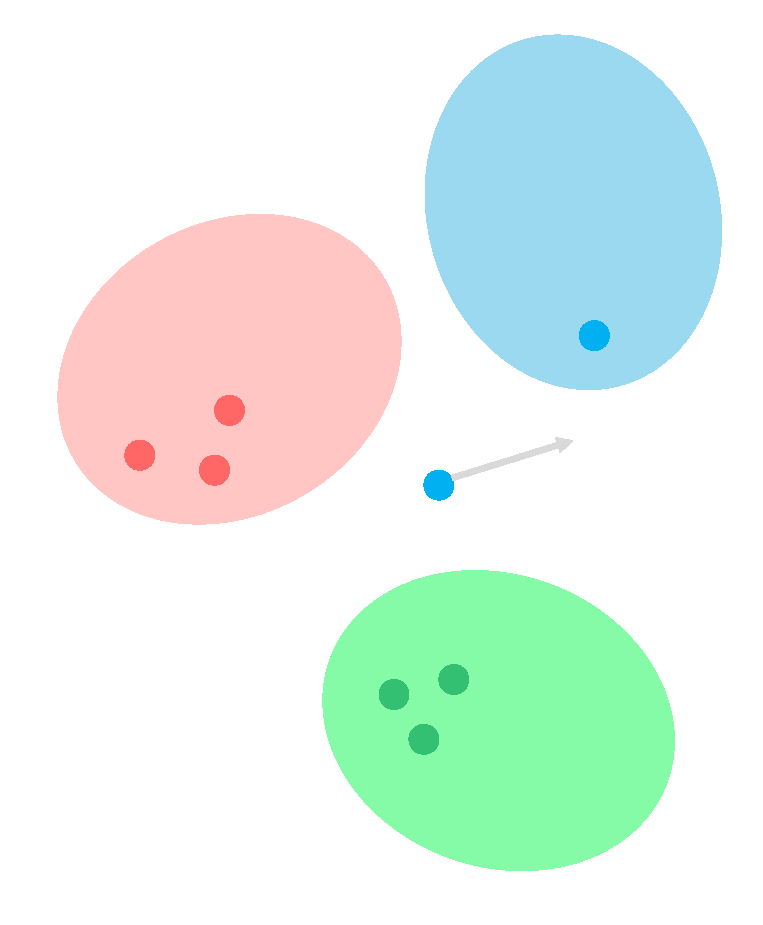
\includegraphics[width=1\linewidth]{figures/in-batch.drawio.pdf}
%         \caption{in-batch}
%         \label{fig:in-batch}
%     \end{subfigure}
%     \begin{subfigure}[t]{0.25\linewidth}
%         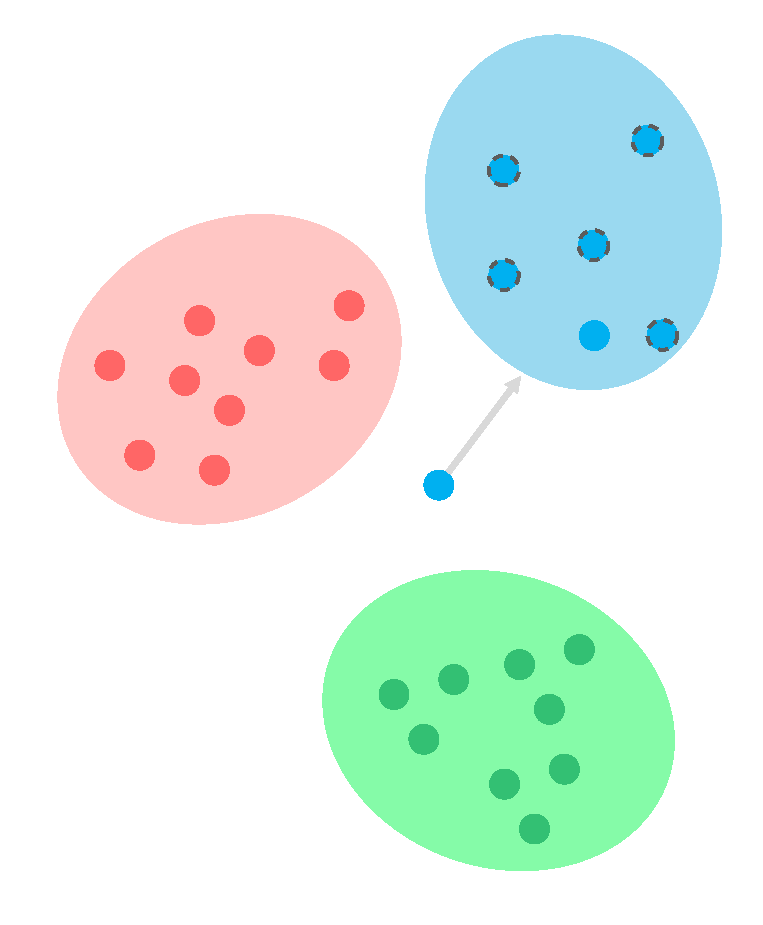
\includegraphics[width=1\linewidth]{figures/large-batch.drawio.pdf}
%         \caption{large batch}
%         \label{fig:large-batch}
%     \end{subfigure}
%     \begin{subfigure}[t]{0.25\linewidth}
%         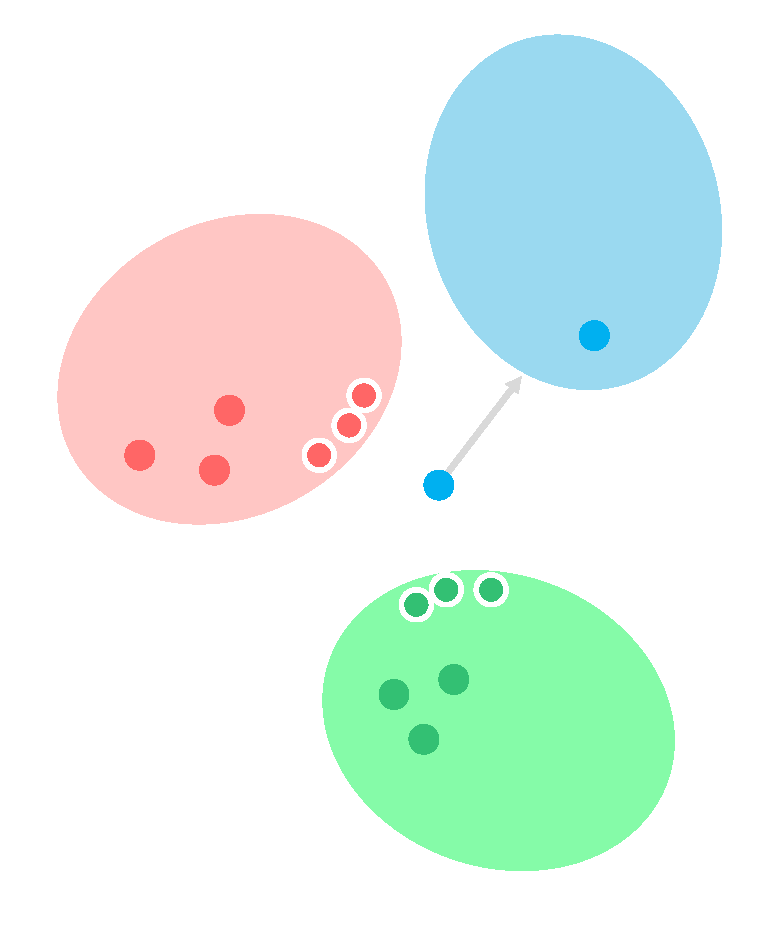
\includegraphics[width=1\linewidth]{figures/hard-negatives.drawio.pdf}
%         \caption{hard negatives}
%         \label{fig:hard-negatives}
%     \end{subfigure}
%     \centering
%     \caption{Negative sampling. Conceptual view on contrastive learning.}
% \end{figure}

It is most effective to train embeddings using supervised positive pairs. For instance, datasets in the domains of natural language inference (NLI), question answering (QA), fact verification, and paraphrases contain pairs of semantically similar texts, making them suitable for training text embeddings \cite{li2023general}. This data is exceptionally clean but limited in quantity. Another approach involves scraping data from web pages, such as QA forums (e.g., Quora) and social media platforms (e.g., Reddit). This data is abundant, but can be noisy. When there are no readily available resources like supervised or scraped pairs, augmentation remains a viable option. In this case, two augmented views of the same object should preserve the essential semantics of the object while posing a challenging task for a model to discriminate one positive sample from the rest of the negative ones. 

Present-day SoTA text embeddings such as BGE \cite{xiao2023cpack}, GTE \cite{li2023general}, E5 \cite{wang2022text} follow the same pipeline of training. First, a retrieval-oriented language model is trained \cite{xiao2022retromae, gao-callan-2021-condenser}, that is a BERT-like model that can efficiently aggregate global information about input sequence. Second, a general-purpose fine-tuning process is conducted using a large corpus of weakly supervised text pairs with large-batch contrastive learning. Finally, task-specific fine-tuning on supervised text pairs occurs employing contrastive learning with hard negative samples.

\subsection{Similar Approaches}

\textbf{Text embedding.} Several existing text embedding methods employ contrastive learning with augmentation-mined positive and negative pairs. CERT \cite{fang2020cert} utilizes back-translation to mine positive pairs, while ConSERT \cite{yan-etal-2021-consert} employs various augmentations at the token level. Doc2vecC \cite{luo2021unsupervised} relies on thesaurus-based augmentations and back-translation for its approach.

\textbf{Dialogue embedding.} Dial2vec \cite{liu2022dial2vec} and DialogueCSE \cite{liu2021dialoguecse} modify transformer architecture by adding cross-attention between different groups of utterances after all transformer layers. To get a positive pair, both works employ the idea of self-guidence that is similar to ours, because they get two views of the same object. In Dial2vec, it's local vs. global information about a dialogue, whereas in DialogueCSE, it's the utterances of the first interlocutor vs. the utterances of the second interlocutor.

Our approach stands apart from the methods mentioned above for the following reasons:
\begin{itemize}
    \item Our set of augmentations is more potent than the one employed in CERT, comprising a comprehensive set of transformations that facilitate the creation of non-obvious examples, beyond mere paraphrasing.
    \item Our augmentations adhere to the set of valid objects, preserving grammatical and meaningful constructs. They do not disrupt the structure of the dialogue, as they are meticulously designed with context-aware language models, unlike ConSERT, which employs simple token shuffling and deletion, retaining only lexical information.
    \item our approach does not modify BERT architecture
\end{itemize}

TODO: add text about SimCLR?

\section{Method}

In this section, we describe our method. It can be divided into two stages. At the first stage, we develop and make augmentations for dialogue data. In result, the dataset consists of samples with following schema: original dialogue, set of augmentations with preserved intents, set with corrupted intents. At the second stage, we apply the contrastive learning.

\subsection{Augmentations} \label{sec:aug}

\textbf{Token Insertion.} One of the simple yet effective ways to augment text is to lengthen it by inserting extra tokens. For this purpose, we added a special token \texttt{<mask>} to random places in the dialogues and used transformer models trained on the MLM task \cite{devlin2019bert} to fill these masks. Insertion is rejected if the token proposed by the model is only a fragment of a word \cite{wu2016googles, sennrich-etal-2016-neural} or if the prediction probability is below a manually set threshold. To take the dialogue context into account during token insertion, multiple consecutive responses were fed into the mask-filling model at once as a compromise between feeding single utterances and entire dialogue.

\textbf{Token Replacement.} This method is identical to the previous one, except that instead of adding the \texttt{<mask>} token, some tokens in the original dialogue are replaced. In this case, the mask-filling model is fed with single utterances to make replacements more diverse and random.

\textbf{Back Translation.} Translation from the original language to another language and then back to the original language. Neural machine translation models were used for this purpose \cite{TiedemannThottingal}.

\textbf{Shuffling Utterances.} Previous augmentations modify the dialogue within a single utterance, since they are methods applicable to arbitrary text data. It seems essential to learn how to change the order of utterances in a dialogue to create new valid dialogue. For this purpose, we propose using a model that measures the similarity between utterances within a dialogue. Using these similarities, it is possible to cluster utterances within each dialogue. Experiments showed that these clusters represent significant individual stages of the dialogue that can be shuffled with each other.

\textbf{Shortening Dialogue.} Individual clusters of utterances within the dialogue can be discarded, resulting in a pruned dialogue with fewer utterances.

\textbf{Lengthening Dialogue.} The special model was trained to arrange a list of given utterances. This transformer takes the text embeddings of each utterance as input sequence, without specifying information about their order in the original dialogue. It outputs ranks that can be used to "sort" the utterances to restore the original order. If some external responses are added to the original dialogue, this model generates a new, longer dialogue.

The augmentations mentioned above can be configured to either preserve or alter intent. Specifically, token replacement can be viewed as intent-corrupting augmentation, because all the keywords such as "restaurant", "taxi" etc. tend to be replaced. Pruning dialogue may remove some intents, but the result is still much similar to original dialogue, since its intents are fully encompassed by the original dialogue's intents. 
Shuffling utterances doesn't change any intents, it only changes their order. The rest of augmentations preserves intents because they either perform paraphrasing (back translation), or add new information (token insertion, lengthening dialogue).

To expand the set of augmentations even further, we use a composition of several ones. For more details on augmentation implementations, please refer to Appendix \ref{app:aug}.

\subsection{Encoder Fine-tuning}

As a model for embedding, we try BERT-like models without any modifications \cite{devlin2019bert}. The input is \texttt{[CLS] ut1 [SEP] ut2 [SEP] ut3}, and the output is the hidden state of \texttt{[CLS]} token from the last layer. 

Also, we experiment with a slightly advanced dialogue language model, HSSA \cite{zhang-etal-2023-dialog}. It uses BERT as a backbone and modifies its attention mechanism to capture the hierarchical structure of dialogue and reach the computational trade-off between feeding a transformer separate utterances and feeding an entire dialogue.

In our fine-tuning, a positive pair is obtained with intent-preserving augmentations of the same dialogue, and the remaining dialogues from the training batch are used as negative samples. In order to reduce required batch size, we utilize intent-corrupting augmentations as hard negative samples.

\subsection{Evaluation} \label{sec:evaluation}

We evaluate dialogue embeddings in transfer learning setting. Specifically, our evaluation methods utilize frozen embeddings as features. Inspired by \cite{liu2022dial2vec} we employ these evaluation methods: 1) domain classification, 2) dialogue retrieval, 3) intent similarity. Evaluation is performed on MultiWOZ 2.2 dataset \cite{zang2020multiwoz}.

\textbf{Domain classification.} The goal is to predict in which domain a dialogue is taking place. In dataset there are 7 domains: attraction, bus, hospital, hotel, restaurant, taxi, train. Each dialogue can take place in multiple domains at once. The method is to train a linear classifier upon dialogue embedding, this is the so-called linear probe evaluation, that is used in many works. F1-macro is used to measure quality. This evaluation method can demonstrate how well embeddings encode some implicit features about the dialogue and its participants in perspective.

\textbf{Dialogue retrieval.} For each dialogue from validation split, the goal is to retrieve dialogues from train split with at least one domain in common. Ranking score is calculated as cosine similarity between query and answer embeddings. Mean average precision at 100 is used to measure quality. This evaluation method can demonstrate potential effectiveness for retrieval and other downstream tasks like clustering.

\textbf{Intent similarity.} We sample pairs of dialogues from train and validation splits of dataset. A linear regression is trained on the former pairs and evaluated on the latter pairs using Pearson correlation between predicted similarity scores and gold ones. The gold scores are obtained using DGAC clustering \cite{dgac}. Clusters represent intents of dialogue participants. Each dialogue can be associated with a set of intents. We define gold intent similarity of two dialogues as a dice similarity between their sets of intents.

\section{Experiments}

this section is incomplete

\textbf{Dataset.} Large dataset is important for contrastive learning. In all experiments, we used the same dataset of dialogues. This dataset is a combination of several task-oriented dialogue datasets from DialogStudio \cite{zhang2023dialogstudio} which are listed in Table \ref{tab:dataset}. All the dialogues were filtered based on their length, resulting in a dataset comprising 501K dialogues.

\begin{table}[!htb]
    \centering
    \begin{tabular}{c|c|c|c}
        Name & \# dialogues & \# utterances & \# tokens \\
        \hline
        AirDialogue & 321K & 4086K & 49.4M \\
        SimJointGEN & 100K & 1584K & 22.5M \\
        MS-DC & & & \\
        MetaLWOZ & & & \\
        MULTIWOZ2\_2 & & & \\
        SGD & & & \\
        KETOD & & & \\
        FRAMES & & & \\
        Disambiguation & & & \\
        ABCD & & & \\
        AirDialogue & & & \\
        BiTOD & & & \\
        Taskmaster1 & & & \\
        \textbf{Total} & & & \\
        \textbf{Filtered} & 501K & 6320K & 83.7M
    \end{tabular}
    \caption{All the datasets are taken from DialogStudio collection \cite{zhang2023dialogstudio}. BERT tokenizer is used to count \# tokens column.}
    \label{tab:dataset}
\end{table}


First, we evaluate pre-trained models BERT \cite{devlin2019bert}, RoBERTa \cite{liu2019roberta}, RetroMAE \cite{xiao2022retromae}. Results are presented in Table \ref{tab:eval-raw}. This table describes existing results, that can be obtained by available model weights without any fine-tuning on dialogue data. 

\begin{table}[!htb]
    \centering
\begin{tabular}{l|c|c|c}
         & Classification & Retrieval & Similarity \\ \hline
BERT     & $47.53$          & $66.31$     &            \\
RoBERTa  & $48.66$          & $84.40$     &            \\
RetroMAE & $69.84$          & $86.95$     &            \\
\end{tabular}
    \caption{Evaluation of available models. For the meaning of these values, see Section \ref{sec:evaluation}.}
    \label{tab:eval-raw}
\end{table}

\textbf{(Weak) Training.} In our fine-tuning approach, we used the following settings: a batch size of 32, AdamW optimizer with a weight decay of 1e-2, and a fixed learning rate of 3e-6. We froze all transformer layers except the last one. It's worth noting that we applied only a partial set of augmentations and worked with just 10\% of the entire dataset. Evaluation results after one epoch of our contrastive fine-tuning on dialogue data are presented in Table \ref{tab:eval-one-epoch}.

\begin{table}[!htb]
    \centering
\begin{tabular}{l|c|c|c}
         & Classification & Retrieval      & Similarity \\ \hline
BERT     & $67.18$ $(+19.65)$ & $77.99$ $(+11.68)$ &            \\
RoBERTa  & $68.20$ $(+19.54)$ & $79.94$ $(-4.46)$  &            \\
RetroMAE & $70.33$ $(+0.49)$  & $89.08$ $(+2.13)$  &           
\end{tabular}
    \caption{Evaluation after one epoch of contrastive fine-tuning. Number in parentheses is a difference with results in Table \ref{tab:eval-raw}. For the meaning of these values, see Section \ref{sec:evaluation}.}
    \label{tab:eval-one-epoch}
\end{table}

\section{Limitations.}

Out method has several limitations.

\begin{itemize}
    \item The weights obtained are specific to the language used. Consequently, it is necessary to gather dialogues in the target language, train auxiliary pairwise and listwise models, and subsequently employ contrastive fine-tuning on a BERT-like encoder. An alternative approach to address this challenge is to accumulate multilingual data.
    \item All experiments were conducted with a complete dialogue inputted directly into the transformer, which is constrained by the maximum number of tokens in the input sequence. One potential resolution is to utilize the HSSA model, designed for handling individual utterances. However, this option may result in a reduction in quality.
\end{itemize}

\section{Conclusion.}

A study has been conducted on building embeddings for task-oriented dialogues. A procedure for contrastive learning with augmentations that preserve and corrupt interlocutors' intents was proposed. The effectiveness of this procedure was demonstrated for BERT-like models in tasks such as dialogue classification, retrieval, and similarity. An ablation study was conducted, showing the contribution of each type of augmentation to the final embeddings.



%Bibliography
\bibliographystyle{unsrt}  
\bibliography{references}  

\appendix

\section{Auxiliary Models} \label{app:aug}

As mentioned in Section \ref{sec:aug}, we trained special models to perform dialogue-level augmentations.

\begin{figure}[!htb]
    \centering
    \begin{subfigure}[t]{0.6\linewidth}
        \centering
        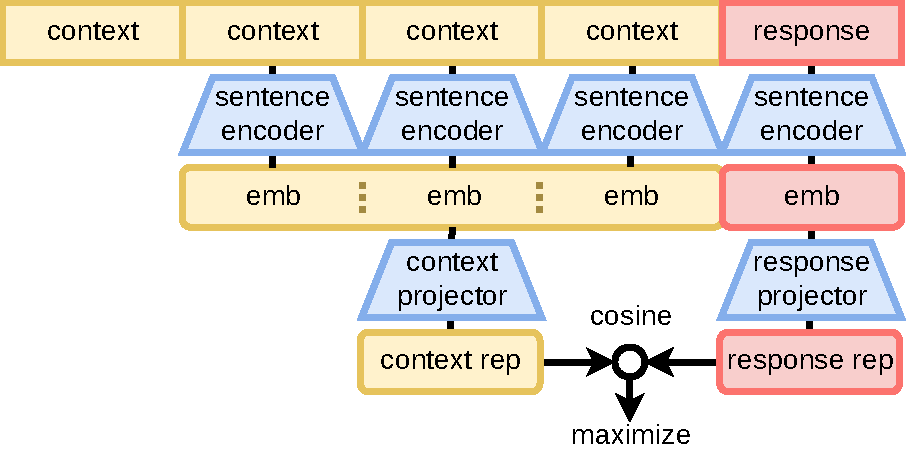
\includegraphics[width=0.9\linewidth]{figures/pairwise.drawio.pdf}
        \caption{for measuring similarity between utterances}
        \label{fig:pairwise}
    \end{subfigure}
    \begin{subfigure}[t]{0.35\linewidth}
        \centering
        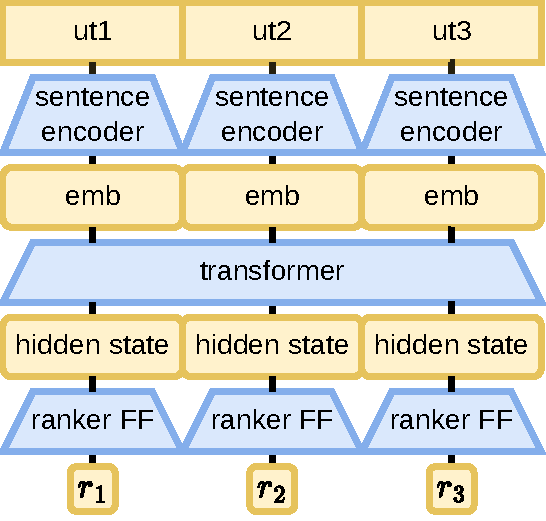
\includegraphics[width=0.9\linewidth]{figures/listwise.drawio.pdf}
        \caption{for lengthening dialogue}
        \label{fig:listwise}
    \end{subfigure}
    \caption{Auxiliary models for performing augmentations.}
    \label{fig:enter-label}
\end{figure}

\subsection{Pairwise Model}

We utilized a model for measuring the similarity between dialog utterances. In its basic form, it can be implemented as follows: take sentence embeddings of the utterances and compare the cosine similarities between them. Training such a model on sequential utterances using contrastive learning yields commendable utterance embeddings \cite{Zhou2022}.

However, this approach has a significant drawback; it does not consider the context from several preceding utterances. In a dialogue, it is crucial to compare not just pairs of utterances but pairs of context-response. Therefore, we employed the following model (Fig. \ref{fig:pairwise}):

\begin{enumerate}
    \item  First, embeddings for all context utterances $c=[u_1,\ldots,u_k]$ and the response $r$ are obtained using a pretrained sentence encoder.
    \item The embeddings of the context are concatenated and passed to a projector that outputs a vector representing the context.
    \item The response embedding is fed into a second encoder, resulting in a vector representing the response.
    \item The cosine similarity between the obtained vectors is computed as a measure of the context and response similarity.
\end{enumerate}

\texttt{aws-ai/dse-bert-large} model from hugging face \cite{wolf2020huggingfaces} was used as the sentence encoder. The model was trained with a contrastive loss using in-batch negative sampling, with the following parameters: batch size is 128, temperature is 0.05, context size is 3, projection size is 256. Only 3 last layers of sentence encoder were fine-tuned in order to decrease computational cost. Trained model reaches 0.955 retrieval accuracy@5. 

Batches were formed from "context-response" pairs from the entire dialog dataset, where negative examples were not samples from the same dialog but entirely random examples from the dataset. This allows batching of arbitrary sizes, not limited to the dialog size, making the pre-training task more challenging.

The resulting model closely resembles the ConveRT model \cite{henderson2020convert} for obtaining utterance embeddings. The drawbacks of the latter model are, firstly, that it is proprietary, and secondly, its architecture is highly specific and does not utilize the familiar BERT-like backbone.

\begin{figure}[!htb]
    \centering
    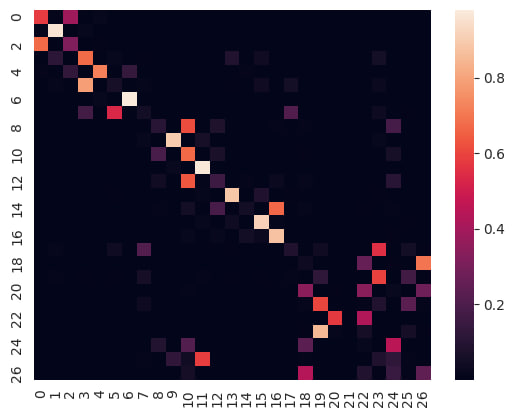
\includegraphics[width=0.5\linewidth]{figures/pairwise-cluster-heatmap.jpg}
    \caption{All similarities between contexts and responses within a dialogue. It is easy to see, that consecutive utterances form clusters.}
    \label{fig:pairwise-clister-heatmap}
\end{figure}

As a result, the obtained model is capable of recognizing individual stages in dialogues (Fig. \ref{fig:pairwise-clister-heatmap}). This behavior is achieved due to two factors. Firstly, when a dialogue furthers to a new topic, the similarity between two consecutive utterances drops substantially. This is clearly visible, for example, in dialogues in which ordering a taxi replaces booking a table in a restaurant. Secondly, within one topic, there are also small drops in similarity in cases where there is a transition from one question to another. For example, the question “how many people should I book for?” replaces the question “which restaurant do you prefer?”. Moreover, since these questions relate to one topic, they remain close to themselves and distant to questions on other topics. Therefore, clusters are obtained.

(!provide the dialogue and change pic to vector instead of raster!)

\subsection{Listwise Model}

We trained the special model to merge utterances of two different dialogues (Fig. \ref{fig:listwise}). It is a transformer over text embeddings of the utterances. Sentence encoder is \texttt{sentence-transformers/all-mpnet-base-v2} from hugging face. We used 4-layer transformer with 4 attention heads and hidden dimension twice smaller than sentence encoder's one, i.e. 384. Only 3 last layers of sentence encoder were fine-tuned in order to decrease computational costs.

Output ranks are transformed with softmax function. Then KL-divergence between output and target probabilities are minimized. Target probabilities are defined as softmax over true ranks of utterances, i.e. $-i$ for $i$-th utterance in dialogue.

Resulting model trains to "sort" given utterances. Thanks to the attention mechanism of transformers, this can be viewed as asking the children at physical education class to look at each other and line up by height.

To measure the sorting quality, we need to utilize appropriate metric. All traditional ranking metrics such as nDCG are designed to compare with gold ranks, not just sorting quality. So during validation of our model, we were converting the ranks to a permutation over the original sequence of $n$ elements. Then, we calculated the number of transpositions. It is easy to implement and can normalized by maximum possible number of transpositions $n(n-1)/2$, resulting in $[0,1]$-ranged metric. Our trained model reaches $0.96$ value.

\section{Composition of Augmentations}

In order to maximize diversity of training data, we use not only 5 basic augmentations described in section \ref{sec:aug}, but also 4 extra compositions of augmentations. All the resulting pipelines are defined in Fig. \ref{fig:aug-compositions}. 

\begin{figure}[!htb]
    \centering
    \begin{subfigure}[t]{0.5\linewidth}
        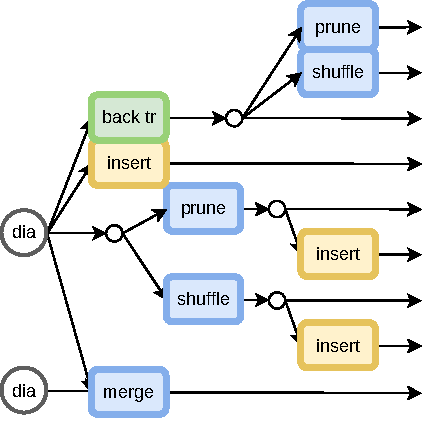
\includegraphics[width=0.85\linewidth]{figures/augmentation-pipeline-positive.drawio.pdf}
        \caption{intent-preserving}
        \centering
    \end{subfigure}
    \begin{subfigure}[t]{0.35\linewidth}
        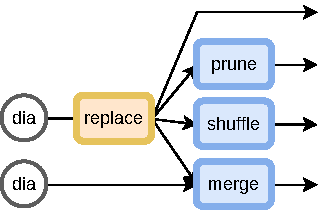
\includegraphics[width=0.9\linewidth]{figures/augmentation-pipeline-negative.drawio.pdf}
        \caption{intent-corrupting}
        \centering
    \end{subfigure}
    \caption{Compositions of augmentations.}
    \label{fig:aug-compositions}
\end{figure}

\end{document}
